This section defines functional and non-functional requirements for the Condenser tool. It begins with an enumeration of usage scenarios that Condenser could be involved in. These are used to help determine the following requirements.

\subsection{Actors}
\begin{center}
	\begin{figure}[htbp]
		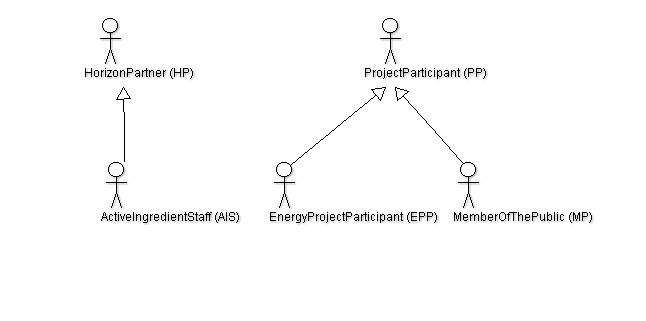
\includegraphics[scale=.5]{images/ActorRelationships.png}
		\caption{Actor relationships.\label{ActorRelationships}}
	\end{figure}
\end{center}	
The actors shown in figure~\ref{ActorRelationships} are involved in the following usage scenarios and cases. They include:
\begin{itemize}
	\item Horizon project staff (HPS) -- These actors are involved in research projects as investigators.
	\item Horizon Partner (HP) -- These actors are involved in research projects as investigators. 
	\item Active Ingredient staff (AIS) -- These actors are a type of Horizon Partner. 
	\item Project Participant (PP) -- These actors are involved in research projects as participants. 
	\item Member of the public (MP) -- These actors are a type of Project Participant recruited from the general public.
	\item Energy project participant (EPP) -- These actors are a type of Project Participant recruited in particular for energy projects.
\end{itemize}

\subsection{Usage Scenarios}
			\subsubsection{Relate Project: Condenser Installation}
			\textbf{Participating Actors:}  Anne:AIS , Harry:HPS \\
\textbf{Event Flow:}
	\begin{enumerate}
\item  Anne prepares to run an energy and climate data collection exercise in the Brazilian rain forest using open mobile sensing kits (OMSK).
\item  Harry installs Condenser on the local server component of the OMSKs.
\item  Harry configures a Cloud-server to accept data uploads from each OMSK.
\item  Harry uses the Condenser RESTful interfaces to configure them to log the data from their local stores to the cloud when connectivity is available. He also configures them to run in low-powered mode by setting their reconnection attempts to a low amount and to only send data in aggregated bursts every hour.
	\end{enumerate}
	\line(1,0){350}
			\subsubsection{Relate Project: Oasis of Connectivity}
			\textbf{Overview:} Condenser's behaviour in long period without connectivity \\
			\textbf{Participating Actors:}  Anne:AIS, Miguel:MP \\
\textbf{Event Flow:}
	\begin{enumerate}
\item Anne conducts a public art activity in the Brazilian rain forest.
\item Anne gives Miguel an OMSK.
\item Miguel activates the OMSK as part of the activity.
\item On start up the OMSK activates Condenser and begins to capture temperature, humidity, C02 and energy information.
\item No network connectivity is available to Condenser so it evaluates the expected data load and determines that no action needs to occur until the next connection attempt. [Note that this would be much more complicated if Condenser determined that the current data capture rates exceeded the storage capacity ]
\item Miguel returns the OMSK to Anne, and she returns to her office with it.
\item \textbf{Condenser} successfully attempts to connect to the network after its timeout. 
\item \textbf{Condenser} transfers the data from the OMSK to the Cloud-store.
\item Anne looks at the day's data using the web-based visualisation tools. These have immediate access to the Cloud-data.
	\end{enumerate}
	\line(1,0){350}	
	\subsubsection{Energy Project: Trickle of Connectivity}
			\textbf{Overview:} Condenser's behaviour during intermittent connectivity \\
			\textbf{Participating Actors:}  Harry:HPS, Ernie:EPP \\
\textbf{Event Flow:}
	\begin{enumerate}
\item Harry is conducting an energy study.
\item Harry sets up a Shiva Plug computer with an energy monitor.
\item Harry installs Condenser on the Shiva Plug.
\item Harry configures Condenser to attempt to reconnect whenever possible and to send discrete data points to a rack-mounted server using particular authentication details. 
\item  Harry installs the energy monitor in Ernie's home and configures it to use Ernie's home router.
\item \textbf{Condenser} attempts to transmit data as the energy monitor receives them, but connectivity is intermittent owing to Ernie's unstable Internet connection.
	\end{enumerate}
	\line(1,0){350}
\subsection{Use Cases}
	\subsubsection{Installation}		 
		Install local server and DB\\	 
		\textbf{Participating Actors:}  ... \\
		\textbf{Event Flow:}
		\begin{enumerate}
\item  ...
	    \end{enumerate}
		\textbf{Entry Conditions:}\\
		\textbf{Exit Conditions:}\\
		\textbf{Quality Requirements:}\\
		\line(1,0){350}		
		
		Set external storage connection settings\\ 
		\textbf{Participating Actors:}  ... \\
		\textbf{Event Flow:}
		\begin{enumerate}
\item  ...
	    \end{enumerate}
		\textbf{Entry Conditions:}\\
		\textbf{Exit Conditions:}\\
		\textbf{Quality Requirements:}\\
		\line(1,0){350}		
		 
		Setup local database \\		 
		\textbf{Participating Actors:}  ... \\
		\textbf{Event Flow:}
		\begin{enumerate}
\item  ...
	    \end{enumerate}
		\textbf{Entry Conditions:}\\
		\textbf{Exit Conditions:}\\
		\textbf{Quality Requirements:}\\
		\line(1,0){350}
						 
		Setup logging \\		 
		\textbf{Participating Actors:}  ... \\
		\textbf{Event Flow:}
		\begin{enumerate}
\item  ...
	    \end{enumerate}
		\textbf{Entry Conditions:}\\
		\textbf{Exit Conditions:}\\
		\textbf{Quality Requirements:}\\
		\line(1,0){350}
						 
		Setup server metadata \\
		\textbf{Participating Actors:}  ... \\
		\textbf{Event Flow:}
		\begin{enumerate}
\item  ...
	    \end{enumerate}
		\textbf{Entry Conditions:}\\
		\textbf{Exit Conditions:}\\
		\textbf{Quality Requirements:}\\
		\line(1,0){350}
				 
		Register nodes	\\	 
		\textbf{Participating Actors:}  ... \\
		\textbf{Event Flow:}
		\begin{enumerate}
\item  ...
	    \end{enumerate}
		\textbf{Entry Conditions:}\\
		\textbf{Exit Conditions:}\\
		\textbf{Quality Requirements:}\\
		\line(1,0){350}
		
	\subsubsection{Local data Capture}		 
		Capture Data\\	 
		\textbf{Participating Actors:}  ... \\
		\textbf{Event Flow:}
		\begin{enumerate}
\item  ...
	    \end{enumerate}
		\textbf{Entry Conditions:}\\
		\textbf{Exit Conditions:}\\
		\textbf{Quality Requirements:}\\
		\line(1,0){350}	
		
		Capture Metadata\\	 
		\textbf{Participating Actors:}  ... \\
		\textbf{Event Flow:}
		\begin{enumerate}
\item  ...
	    \end{enumerate}
		\textbf{Entry Conditions:}\\
		\textbf{Exit Conditions:}\\
		\textbf{Quality Requirements:}\\
		\line(1,0){350}	
		
		Capture Logging Information\\	 
		\textbf{Participating Actors:}  ... \\
		\textbf{Event Flow:}
		\begin{enumerate}
\item  ...
	    \end{enumerate}
		\textbf{Entry Conditions:}\\
		\textbf{Exit Conditions:}\\
		\textbf{Quality Requirements:}\\
		\line(1,0){350}						
	\subsubsection{Data Transfer}		
The following use cases pertain to how Condenser transfers data to the cloud. Figure~\ref{DataTransferUse} shows a diagram depicting the relationships between the data transfer use cases.
\begin{center}
	\begin{figure}[htbp]
		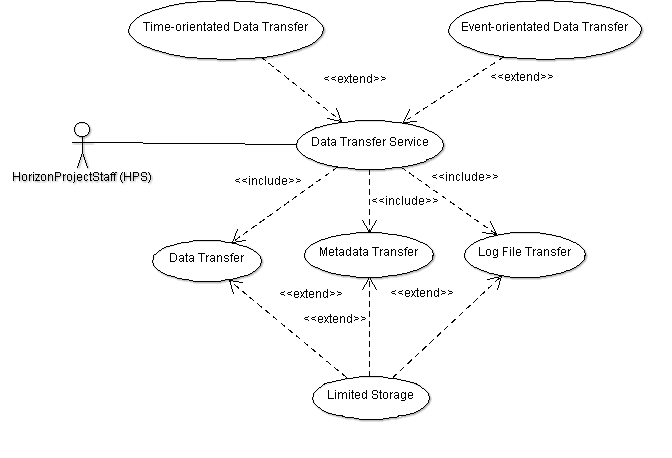
\includegraphics[scale=.5]{images/DataTransferUse.png}
		\caption{Use cases defining Condenser data transfer.\label{DataTransferUse}}
	\end{figure}
\end{center}	
 
		Standard Data Transfer\\	 
		\textbf{Participating Actors:}  ... \\
		\textbf{Event Flow:}
		\begin{enumerate}
\item  ...
	    \end{enumerate}
		\textbf{Entry Conditions:}\\
		\textbf{Exit Conditions:}\\
		\textbf{Quality Requirements:}\\
		\line(1,0){350}			
			 
		Metadata Transfer\\	 
		\textbf{Participating Actors:}  ... \\
		\textbf{Event Flow:}
		\begin{enumerate}
\item  ...
	    \end{enumerate}
		\textbf{Entry Conditions:}\\
		\textbf{Exit Conditions:}\\
		\textbf{Quality Requirements:}\\
		\line(1,0){350}		
			 
		Handling limited data storage concerns \\	 
		\textbf{Participating Actors:}  ... \\
		\textbf{Event Flow:}
		\begin{enumerate}
\item  ...
	    \end{enumerate}
		\textbf{Entry Conditions:}\\
		\textbf{Exit Conditions:}\\
		\textbf{Quality Requirements:}\\
		\line(1,0){350}		
	\subsubsection{Local Service Review}		 
	Metadata Review \\	 
	\textbf{Participating Actors:}  ... \\
	\textbf{Event Flow:}
	\begin{enumerate}
\item  ...
    \end{enumerate}
	\textbf{Entry Conditions:}\\
	\textbf{Exit Conditions:}\\
	\textbf{Quality Requirements:}\\
	\line(1,0){350}		
			 
	Log Review \\	 
	\textbf{Participating Actors:}  ... \\
	\textbf{Event Flow:}
	\begin{enumerate}
\item  ...
    \end{enumerate}
	\textbf{Entry Conditions:}\\
	\textbf{Exit Conditions:}\\
	\textbf{Quality Requirements:}\\
	\line(1,0){350}			
	\subsubsection{Decommissioning}		 
The following use cases pertain to the decomissioning of Condenser components. Figure~\ref{DecomissioningUse} shows a diagram depicting the relationships between the decomissioning use cases.
\begin{center}
	\begin{figure}[htbp]
		%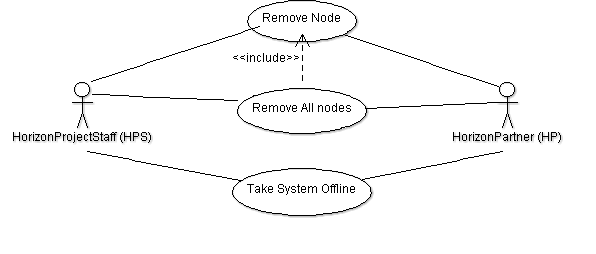
\includegraphics[scale=.5]{images/DecomissioningUse.png}
		\caption{Use cases defining Condenser decomissioning.\label{DecomissioningUse}}
	\end{figure}
\end{center}	
\textbf{Use Cases:}\\

	\textbf{Removing a node} \\	 
	\textbf{Participating Actors:} Horizon Project Staff(HPS) and/or Horizon Partner (HP) \\
	\textbf{Event Flow:}
	\begin{enumerate}
\item HPS or HP accesses the node registry web interface for the given device. 
\item HPS or HP un-subscribes to a node.
\item Condenser ceases to receive data from the node.
	    \end{enumerate}
		\textbf{Entry Conditions:} A node is registered with Condenser.\\
		\textbf{Exit Conditions:} The node is no longer registered with Condenser.\\
		\line(1,0){350}

	\textbf{Removing all nodes} \\	 
	\textbf{Participating Actors:}  Horizon Project Staff(HPS) and/or Horizon Partner (HP) \\
	\textbf{Event Flow:}
	\begin{enumerate}
\item HPS or HP accesses the node registry web interface for the given device. 
\item HPS or HP un-subscribes all nodes.
    \end{enumerate}
	\textbf{Entry Conditions:} At least one node is registered with Condenser.\\
	\textbf{Exit Conditions:} No nodes are registered with Condenser.\\
	\line(1,0){350}		

	\textbf{Taking Condenser offline} \\	 
	\textbf{Participating Actors:}  Horizon Project Staff(HPS) and/or Horizon Partner (HP) \\
	\textbf{Event Flow:}
	\begin{enumerate}
\item HPS or HP accesses the uninstall web interface for the given device. 
\item After a suitable warning HPS or HP initiate unistall.
\item Condenser attempts to backup all outstanding data, metadata and longs.
\item Condenser removes its local data storage contents and schema.
\item Condenser removes all of its installed software.
    \end{enumerate}
	\textbf{Entry Conditions:} Condenser is running.\\
	\textbf{Exit Conditions:}\\	
	\begin{enumerate}
\item All data cached by Condenser is replicated elsewhere.
\item Condenser is uninstalled leaving no footprint.
    \end{enumerate}
	\line(1,0){350}			
	\subsubsection{Features and Plug-ins}		
The following use cases pertain to advanced features of Condenser. Figure~\ref{FeaturesAndPluginsUse} shows a diagram depicting the relationships between the features and plug-ins use cases.
\begin{center}
	\begin{figure}[htbp]
		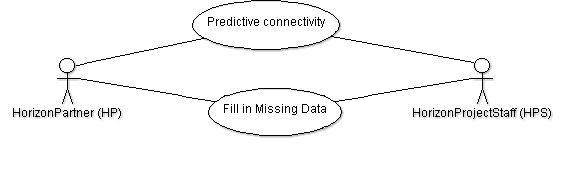
\includegraphics[scale=.5]{images/FeaturesAndPluginsUse.png}
		\caption{Use cases defining Condenser advanced features.\label{FeaturesAndPluginsUse}}
	\end{figure}
\end{center}	
\textbf{Use Cases:}\\

	\textbf{Predictive connectivity} \\	 
	\textbf{Participating Actors:}  ... \\
	\textbf{Event Flow:}
	\begin{enumerate}
\item  ...
    \end{enumerate}
	\textbf{Entry Conditions:}\\
	\textbf{Exit Conditions:}\\
	\textbf{Quality Requirements:}\\
	\line(1,0){350}		
 
	\textbf{Filling in missing data} \\	 
	\textbf{Participating Actors:}  ... \\
	\textbf{Event Flow:}
	\begin{enumerate}
\item  ...
    \end{enumerate}
	\textbf{Entry Conditions:}\\
	\textbf{Exit Conditions:}\\
	\textbf{Quality Requirements:}\\
	\line(1,0){350}		

		